\documentclass{article}

\usepackage{neurips_2026}

\usepackage[utf8]{inputenc}
\usepackage[T1]{fontenc}
\usepackage{hyperref}
\usepackage{url}
\usepackage{booktabs}
\usepackage{amsfonts}
\usepackage{amsmath}
\usepackage{nicefrac}
\usepackage{microtype}
\usepackage{xcolor}
\usepackage{graphicx}
\usepackage{array}
\usepackage{enumitem}
\usepackage{placeins}
\usepackage{tikz}
\usetikzlibrary{arrows.meta,positioning}

\newcommand{\method}[1]{\texttt{#1}}

\title{Diagnosing Semantic Navigation with a Four-Stage Decomposition of Memory-Based Place Retrieval}

\author{%
  Anonymous Authors \\
  Anonymous Institution \\
  Anonymous Address \\
  \texttt{anonymous@anonymous.edu} \\
}

\begin{document}

\maketitle

\begin{abstract}
We present a four-stage diagnostic framework for semantic navigation, where the target is a semantic place pattern rather than a coordinate. We decompose memory-based place retrieval into query formation (Q), retrieval satisfaction (R), target materialization (M), and completion after retrieval (C); formalize this probabilistically; and prove that under a conditional stage-Markov assumption the four nested factors are identifiable from trajectories. We instantiate the framework with a symbolic-semantic memory stack and evaluate it on a 10-seed MiniGrid benchmark plus a BabyAI portability check. Targeted oracle interventions close the diagnostic loop counterfactually: hazard recovery responds sharply to oracle retrieval (0.39 $\rightarrow$ 0.60) but only weakly to oracle controller (0.39 $\rightarrow$ 0.43), while goal-region rejoin improves in semantic-path completion without any end-to-end gain. The contribution is a reproducible diagnostic protocol that turns success-only failures into stage-attributable, intervention-guiding measurements.
\end{abstract}

\section{Introduction}

Classical navigation benchmarks often assume that the agent is given an explicit destination coordinate or a dense task reward. Many practical navigation problems are different: the agent must reach a place of a certain \emph{type}, such as a safe rest area, a water-like resource location, a post-hazard recovery exit, or a goal-associated region. Such targets are not naturally specified by a fixed $(x, y)$ waypoint. They are specified by a semantic pattern.

This paper studies a narrower and more diagnostic problem than general embodied intelligence: can a navigation agent choose and reach places defined by semantic patterns rather than coordinates, and can we measure where that process fails? The central claim is methodological. We propose a four-stage diagnostic framework for semantic navigation and use a symbolic-semantic memory stack as one concrete instantiation of that framework. We decompose memory-based place retrieval into four stages: query formation, retrieval satisfaction, target materialization, and completion after retrieval (Q/R/M/C).

This decomposition matters because success-only metrics collapse qualitatively different failures into a single scalar. In our benchmark, water search and safe-rest tasks are already strong end-to-end cases, but goal-region rejoin and hazard recovery are substantially harder. A success-only view would make the whole system look uniformly weak. The four-stage view says something much more useful: goal-region rejoin remains bottlenecked downstream of semantic candidate selection, while hazard recovery remains bottlenecked by retrieval quality itself.

The framing is timely for two reasons. First, embodied and goal-conditioned agents increasingly need to retrieve places, objects, or tools by \emph{meaning} rather than by coordinate \citep{andrychowicz2017hindsight,ghosh2021learning,savva2019habitat}. Second, recent LLM-agent systems increasingly rely on explicit memory layers, yet their evaluation remains mostly success-oriented rather than diagnosis-oriented \citep{wang2023voyager,shinn2023reflexion,packer2023memgpt}. Our contribution is to make semantic navigation measurable at the level of intermediate failures.

Our contributions are: (i) a four-stage diagnostic framework with a probabilistic factorization, (ii) an identifiability result, (iii) a symbolic-semantic instantiation, and (iv) a benchmark with mechanism-targeted assist ablations and oracle interventions. We demonstrate not only that the framework localizes failures, but that these localizations are actionable: targeting the identified bottleneck in isolation yields predictable stage-wise improvement.

\section{Related work}

Our work sits at the intersection of semantic navigation, memory-based RL, and diagnostic evaluation. Classical cognitive-map and semantic-map perspectives motivate explicit place abstractions \citep{tolman1948cognitive,okeefe1978hippocampus,kuipers2000spatial}. In modern embodied AI, learned navigation systems often combine mapping and planning \citep{gupta2017cognitive}, while topological memory methods such as SPTM expose explicit graph structure for navigation \citep{savinov2018semi}. Goal-conditioned RL methods typically condition on explicit goals or embeddings \citep{andrychowicz2017hindsight,ghosh2021learning}, and successor-representation work provides another route to predictive structure \citep{dayan1993improving,stachenfeld2017hippocampus,momennejad2017successor}. Our setting differs in that the target is not a coordinate or latent goal vector supplied by the benchmark, but a semantic pattern that must be retrieved from memory.

Habitat, AI2-THOR, and ProcTHOR made visually rich navigation evaluation standard \citep{savva2019habitat,kolve2017ai2thor,deitke2022procthor}. We deliberately focus on MiniGrid-class environments to obtain clean and reproducible stage measurements, and use BabyAI only as a portability check. Recent LLM-agent systems also emphasize tool use, reflection, and explicit long-term memory \citep{wang2023voyager,shinn2023reflexion,packer2023memgpt}. We do not claim to solve LLM-agent memory here; rather, we argue that the same Q/R/M/C decomposition is a useful template for evaluating memory-grounded agent decisions beyond navigation.

\section{Problem formulation}

At each time step $t$, the agent receives an observation $o_t$ and an internal state summary $s_t$ (for example, hazard phase, thirst, or energy). The navigation problem is not specified by a coordinate goal $g = (x, y)$, but by a semantic intent $I_t$ such as \texttt{find\_water\_source} or \texttt{hazard\_recovery\_exit}. The intent induces a planner query
\[
q_t = \bigl(I_t, \texttt{required}, \texttt{preferred}, \texttt{penalty}, s_t\bigr),
\]
which is evaluated against a symbolic memory of previously observed places and transitions.

We are interested in semantic-place navigation episodes in which success depends on both \emph{choosing the right kind of place} and \emph{reaching it}. This motivates stage-specific metrics:
\begin{align*}
Q &= \mathbb{1}[\text{query produced a non-empty candidate set}],\\
R &= \mathbb{1}[\text{retrieved candidate satisfied the semantic query}],\\
M &= \mathbb{1}[\text{candidate was materialized into an actionable target}],\\
C &= \mathbb{1}[\text{episode succeeded after retrieval}].
\end{align*}

The central empirical question is therefore not just whether the agent succeeds, but \emph{which stage fails first} when it does not. We use two related measurement layers. \textbf{Operational rates} count, per query attempt, whether the query yielded a non-empty candidate set, whether the chosen candidate satisfied the semantic predicate, and whether it was materialized into an actionable target; \emph{completion after retrieval} is an episode-level indicator. \textbf{Nested episode-level events} $Q^\star \Rightarrow R^\star \Rightarrow M^\star \Rightarrow C^\star$ are used in the factorization of Section~4 and audited in Section~7.1. Full operational definitions are given in Appendix~B.

\section{Theoretical framework}

\subsection{Probabilistic factorization}

Let $Y$ denote overall episode success, and let $Q^\star, R^\star, M^\star, C^\star$ denote the nested episode-level semantic-path events introduced in Section~3 and defined operationally in Appendix~B. Our framework factorizes \emph{semantic-path completion} rather than raw task success:
\[
Q^\star \rightarrow R^\star \rightarrow M^\star \rightarrow C^\star.
\]
For any query $q$ and memory state $\mathcal{M}$, we write
\begin{align*}
P(C^\star = 1 \mid q, \mathcal{M})
&=
P(Q^\star = 1 \mid q, \mathcal{M})\;
P(R^\star = 1 \mid Q^\star = 1, q, \mathcal{M}) \\
&\quad \cdot
P(M^\star = 1 \mid R^\star = 1, q, \mathcal{M})\;
P(C^\star = 1 \mid M^\star = 1, q, \mathcal{M}).
\end{align*}
This factorization is not merely a visualization device; it determines which conditional event is blamed when the semantic pathway fails. Overall task success $Y$ can exceed $C^\star$ because some episodes succeed without traversing the full semantic retrieval path.

\subsection{Identifiability}

\paragraph{Assumption 1 (conditional stage-Markov property).}
Conditioned on the current stage being successful, the probability of the next stage depends only on the current successful stage, the current query, and the current memory state, not on earlier stages directly. Formally,
\[
P(R^\star \mid Q^\star, q, \mathcal{M}, \text{history}) = P(R^\star \mid Q^\star, q, \mathcal{M}),
\]
and analogously for $M^\star$ and $C^\star$.

\paragraph{Assumption 2 (positivity).}
Each conditioning event used above has non-zero probability on the support of the benchmark.

\paragraph{Theorem 1.}
Under Assumptions 1--2, the four stage factors
\[
P(Q^\star=1 \mid q,\mathcal{M}),\;
P(R^\star=1 \mid Q^\star=1,q,\mathcal{M}),\;
P(M^\star=1 \mid R^\star=1,q,\mathcal{M}),\;
P(C^\star=1 \mid M^\star=1,q,\mathcal{M})
\]
are identifiable from trajectory observations. Moreover, the empirical-frequency estimators obtained by counting benchmark events are consistent.

\paragraph{Proof sketch.}
The first claim follows from the chain rule together with the conditional stage-Markov property, which removes dependence on earlier latent history once the current stage is conditioned on. Identifiability then reduces to estimating conditional Bernoulli probabilities on measurable events. Consistency follows from the uniform law of large numbers over finite stage events and the positivity assumption, which ensures non-degenerate denominators. Appendix~A gives the full proof in the same starred notation used by the benchmark. \hfill $\square$

\paragraph{When Assumption~1 may fail.}
Assumption~1 holds tightly here because $q$ and $\mathcal{M}$ are explicitly logged at every stage event. Two practically relevant violations remain: adaptive in-episode query rewrites not surfaced to the logger, and hidden between-stage memory updates. In those cases the factorization should be read as a projection onto observable traces rather than as a full structural identification claim.

\subsection{Mechanism-level interpretation}

The same decomposition also admits a stage-structured mechanism reading. Figure~\ref{fig:causal} treats stage outcomes as a directed acyclic graph. Under this interpretation, assist on/off ablations are best viewed as mechanism-targeted perturbations of materialization and post-retrieval execution rather than as undifferentiated sensitivity analyses.

\begin{figure}[t]
  \centering
  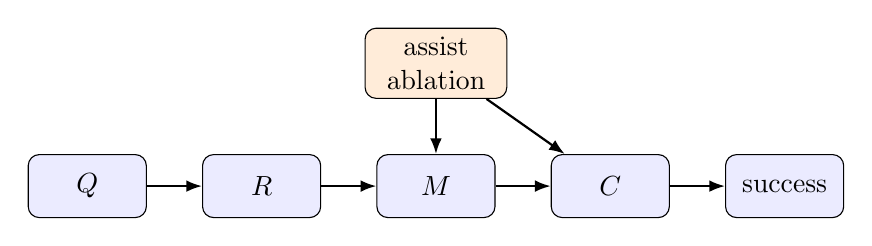
\begin{tikzpicture}[
    node distance=7mm and 7mm,
    box/.style={draw, rounded corners, align=center, minimum height=8mm, minimum width=15mm, fill=blue!8},
    arrow/.style={-{Latex[length=2.0mm]}, thick},
    assist/.style={draw, rounded corners, align=center, minimum height=7mm, minimum width=18mm, fill=orange!15}
  ]
    \node[box] (q) {$Q$};
    \node[box, right=of q] (r) {$R$};
    \node[box, right=of r] (m) {$M$};
    \node[box, right=of m] (c) {$C$};
    \node[box, right=of c] (s) {success};
    \node[assist, above=of m] (a) {assist\\ablation};
    \draw[arrow] (q) -- (r);
    \draw[arrow] (r) -- (m);
    \draw[arrow] (m) -- (c);
    \draw[arrow] (c) -- (s);
    \draw[arrow] (a) -- (m);
    \draw[arrow] (a) -- (c);
  \end{tikzpicture}
  \caption{Stage-structured interpretation of the Q/R/M/C framework. Assist on/off ablations target intermediate mechanisms instead of acting as undifferentiated end-to-end perturbations.}
  \label{fig:causal}
\end{figure}

\section{Symbolic-semantic memory stack}

\subsection{Pipeline overview}

Our system uses a graph substrate but exposes a semantic retrieval interface on top of it. Observations are converted into symbolic scene tokens and semantic tags; these update a memory layer that stores place evidence, episodic traces, transition statistics, and concept/relation records. A planner query is then answered by retrieving candidate places whose semantic profiles match the current task intent and state. Importantly, the same pipeline can be evaluated under the Q/R/M/C framework regardless of the specific retrieval backend.

\begin{figure}[t]
  \centering
  \resizebox{\linewidth}{!}{%
  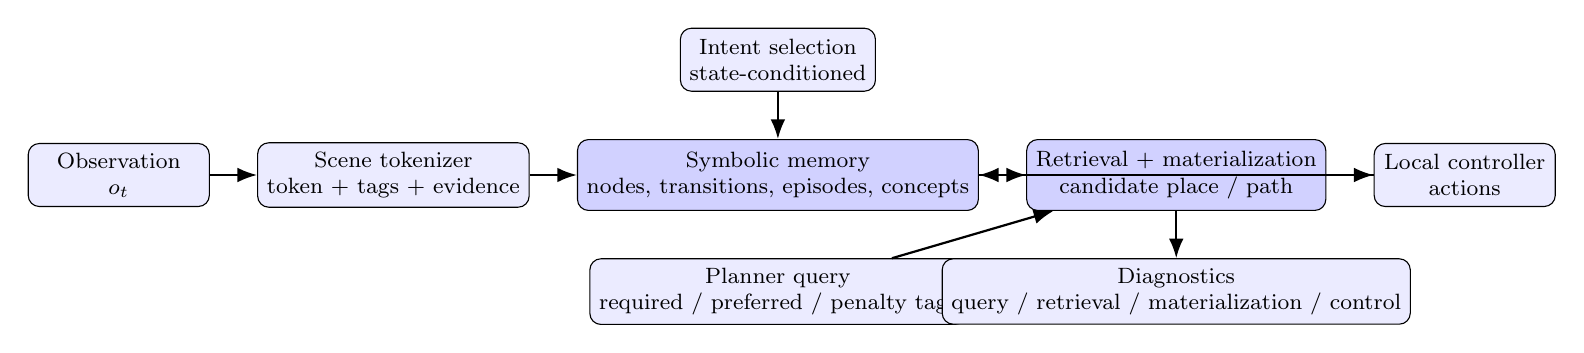
\begin{tikzpicture}[
    node distance=6mm and 6mm,
    font=\footnotesize,
    box/.style={draw, rounded corners, align=center, minimum height=8mm, minimum width=23mm, fill=blue!8},
    darkbox/.style={draw, rounded corners, align=center, minimum height=9mm, minimum width=28mm, fill=blue!18},
    arrow/.style={-{Latex[length=2.5mm]}, thick}
  ]
    \node[box] (obs) {Observation\\$o_t$};
    \node[box, right=of obs] (token) {Scene tokenizer\\token + tags + evidence};
    \node[darkbox, right=of token] (memory) {Symbolic memory\\nodes, transitions, episodes, concepts};
    \node[box, above=of memory] (intent) {Intent selection\\state-conditioned};
    \node[box, below=of memory] (query) {Planner query\\required / preferred / penalty tags};
    \node[darkbox, right=of memory] (retrieval) {Retrieval + materialization\\candidate place / path};
    \node[box, right=of retrieval] (control) {Local controller\\actions};
    \node[box, below=of retrieval] (metrics) {Diagnostics\\query / retrieval / materialization / control};

    \draw[arrow] (obs) -- (token);
    \draw[arrow] (token) -- (memory);
    \draw[arrow] (intent) -- (memory);
    \draw[arrow] (memory) -- (retrieval);
    \draw[arrow] (query) -- (retrieval);
    \draw[arrow] (retrieval) -- (control);
    \draw[arrow] (retrieval) -- (metrics);
    \draw[arrow] (control.west) |- ++(-0.8,0) |- (memory.east);
  \end{tikzpicture}
  }
  \caption{Pipeline overview. The navigation target is generated by semantic retrieval from memory rather than supplied as a coordinate. The pipeline also defines where the Q/R/M/C metrics are measured: query formation at memory/query interaction, retrieval satisfaction at candidate selection, materialization at planner grounding, and completion after retrieval at controller execution.}
  \label{fig:pipeline}
\end{figure}

\subsection{Memory entities}

The memory stores four kinds of records: symbolic place records (per-place semantic tag confidences, counts, visitation, freshness, geometry); transition records (success, risk, and cost statistics with fast/slow estimates); episodic traces (which intent and state were active at each visit); and concept/relation records (higher-level place categories). Detailed schemas are in Appendix~C.

\subsection{Symbol grounding and memory updates}

At each step, the tokenizer emits a symbolic token, semantic tags, and local evidence,
\[
o_t \mapsto (z_t, \tau_t, e_t).
\]
We maintain per-place semantic confidence tables and count statistics over tags using a lightweight online update. A convenient probabilistic interpretation is Dirichlet-multinomial: if place $p$ has tag counts $\mathbf{n}_p$ and prior concentration $\boldsymbol{\alpha}$, then after observing evidence for tag $\tau$ one may write
\[
P(\tau \mid p, e_{1:t}) \propto \alpha_\tau + n_{p,\tau}.
\]
Transitions are updated analogously through exponentially smoothed success, risk, and cost statistics, and episodic records attach the current intent and agent state to the visited place so that later retrieval is state-aware rather than purely descriptive.

\subsection{Query semantics}

The planner query supports intent-conditioned retrieval using required, preferred, and penalty tags. The same retrieval machinery is reused across all tasks. We do not introduce a separate planner architecture per task family. The scoring rule used by the retrieval layer is a weighted semantic decision rule:
\[
s(p \mid q_t, s_t)
=
\sum_{\tau \in q_t^{\mathrm{req}}} \log P(\tau \mid p)
\;+\;
\alpha \sum_{\tau \in q_t^{\mathrm{pref}}} \log P(\tau \mid p)
\;-\;
\beta \sum_{\tau \in q_t^{\mathrm{pen}}} \log P(\tau \mid p)
\;+\;
\gamma \, u_{\mathrm{epi}}(p, s_t),
\]
where $u_{\mathrm{epi}}$ is an episodic usefulness term derived from prior outcomes under similar agent states. This makes retrieval a probabilistically interpretable semantic decision rule rather than a task-specific heuristic.

\section{Experimental setup}

\subsection{Tasks, methods, and metrics}

We evaluate four semantic task families --- water search, safe rest, goal-region rejoin (Empty-6x6 and FourRooms), and hazard recovery (LavaGapS7) --- defined by semantic place patterns rather than coordinate goals; full schema is in Appendix~C. The canonical main benchmark uses 10 seeds, 8 episodes per seed, 2 assist modes, and a stabilized baseline roster. We compare node-level semantic retrieval, concept-level retrieval/planning, and state-conditioned variants against four baselines: a random action policy, a graph-only policy without semantic retrieval, an SPTM-like topological baseline built from patch-hash observations, and a learned external behavior-cloned policy trained on oracle-controller demonstrations over full-state observations without symbolic memory. The random baseline samples environment actions uniformly; its non-trivial scores on water/rest reflect the small Empty-6x6 layouts and short horizons rather than any hidden semantic competence, so we treat those tasks mainly as positive-control diagnostics.

We report:
\begin{itemize}[leftmargin=16pt]
\item end-to-end success rate and average steps;
\item query formed rate;
\item retrieval satisfied rate;
\item target materialized rate;
\item completion after retrieval;
\item assist on/off deltas;
\item task-level weakest stage and method-level weakest stage.
\end{itemize}

This evaluation protocol is the main methodological contribution of the work. A system can now be weak end-to-end but still informative scientifically if it exposes a stable failure structure.

\subsection{Protocol}

All reported means are computed over seed-level aggregates. We report 95\% bootstrap confidence intervals using $B=10{,}000$ resamples of seed means. Assist on/off comparisons are evaluated with paired Wilcoxon signed-rank tests over seed-level metrics, with Holm-Bonferroni correction across task families. For transparency, the benchmark runner exports both aggregate rows and episode-level rows, enabling direct recomputation of all statistics and figures.

Each benchmark condition is aggregated at the seed level. Episodes are reset between trials, while the per-run memory state evolves within each seeded benchmark run exactly as logged by the benchmark runner. The assist flags modify only local controller-side support mechanisms: local resource guidance and goal-rejoin fallback behavior. Semantic observations, query logging, and memory updates are otherwise unchanged. All experiments ran on a single 10-core ARM CPU machine with 32\,GB RAM; no accelerator was used. The full benchmark is exported from one source-of-truth runner, and the targeted oracle-intervention sweep reported later (2 task families $\times$ 4 regimes $\times$ 10 seeds $\times$ 8 episodes) completes in under one minute wall-clock.

\subsection{Oracle-stage intervention protocol}

In addition to the observational Q/R/M/C diagnostics, we include a targeted oracle-intervention block on the two hardest task families: goal-region rejoin on \texttt{MiniGrid-FourRooms-v0} and hazard recovery on \texttt{MiniGrid-LavaGapS7-v0}. For each task we compare four regimes: \emph{base}, \emph{oracle retrieval}, \emph{oracle materialization}, and \emph{oracle controller}. Each regime is evaluated over 10 seeds with 8 episodes per seed.

The oracle modes replace exactly one stage-level mechanism while leaving the rest of the pipeline unchanged. Oracle retrieval injects a semantically correct candidate when the semantic pathway is entered. Oracle materialization converts a successful retrieval into an actionable target waypoint. Oracle controller removes downstream execution noise after a materialized target has already been selected. The purpose of this block is not to define a stronger benchmark leaderboard, but to test whether the failure interpretation suggested by the stage profiles survives controlled mechanism replacement. We additionally run a portability check on \texttt{BabyAI-GoToObjMaze-v0} (5 seeds $\times$ 8 episodes); protocol and results are in Appendix~D.

\section{Results}

\subsection{Stage-estimator validation}

Before the main benchmark we validate the factorization. On a synthetic four-stage process with known probabilities the nested-estimator product tracks empirical semantic-path completion across sample sizes (Appendix~E, Fig.~\ref{fig:stage-validation}). On the real benchmark, the same product matches semantic-path completion rather than overall success (Table~\ref{tab:consistency}), confirming that operational rates and nested factors are distinct quantities.

\begin{table*}[t]
  \caption{Stage-factor consistency audit for the best semantic method in each task family. The product of nested conditional estimators matches semantic-path completion, while overall success can be higher because some episodes succeed without traversing the full semantic retrieval path.}
  \label{tab:consistency}
  \centering
  \small
  \begin{tabular}{p{1.7cm}p{2.5cm}c c c c c c c}
    \toprule
    Task & Method & Overall success & Semantic-path completion & $\hat P(Q^\star)$ & $\hat P(R^\star \mid Q^\star)$ & $\hat P(M^\star \mid R^\star)$ & $\hat P(C^\star \mid M^\star)$ & Product \\
    \midrule
    Water & \texttt{water-concept-plan-v1} & 0.95 & 0.70 & 1.00 & 0.98 & 0.74 & 0.97 & 0.70 \\
    Rest & \texttt{rest-state-v2} & 0.93 & 0.73 & 1.00 & 1.00 & 0.80 & 0.91 & 0.73 \\
    Goal region & \texttt{goal-node-v1} & 0.54 & 0.00 & 1.00 & 0.54 & 0.01 & 0.00 & 0.00 \\
    Hazard recovery & \texttt{hazard-state-v7} & 0.40 & 0.16 & 1.00 & 0.56 & 0.58 & 0.50 & 0.16 \\
    \bottomrule
  \end{tabular}
\end{table*}

\subsection{Overall task-family summary}

\begin{figure}[t]
  \centering
  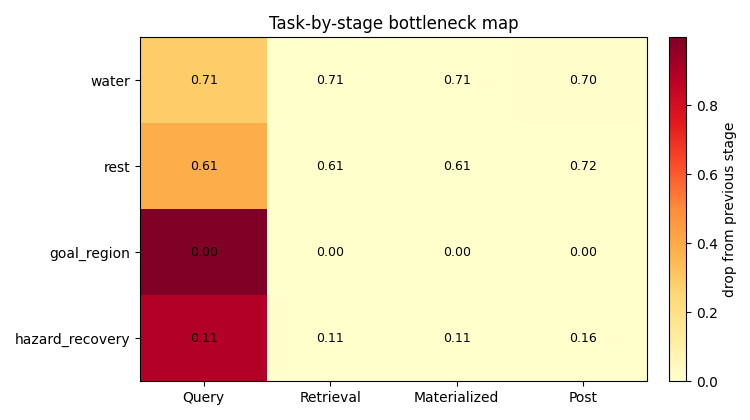
\includegraphics[width=0.88\linewidth]{songlines_symbolic_memory_figures/article_stage_heatmap.png}
  \caption{Hero view of the benchmark: each row is a task family and each column is a stage rate for the best semantic variant. Water and rest remain strong across all stages. Hazard recovery fails early in the pipeline, with retrieval already weak. Goal-region appears flat at zero in the task-family-blended view because the harder FourRooms split dominates the average; the oracle-stage block in Section~\ref{sec:oracle} shows that the failure is downstream of candidate selection rather than a pure query failure.}
  \label{fig:hero-heatmap}
\end{figure}

Table~\ref{tab:main-results} shows the best result found for each task family together with the weakest stage. The stage columns in this table are \emph{operational diagnostic rates}, not the conditional factors from Table~\ref{tab:consistency}. Water and rest are already strong end-to-end tasks. Goal-region and hazard-recovery remain difficult, but the stage decomposition makes the source of difficulty explicit.

\begin{table*}[t]
  \caption{Best semantic result per task family from the final 10-seed benchmark, with 95\% bootstrap confidence intervals on success over seed-level aggregates. The narrow goal-region CI reflects low cross-seed variance because the FourRooms layout is structurally identical across seeds, so per-seed means cluster tightly near 0.54. The query/retrieval/materialized/post-retrieval columns are operational diagnostic rates aggregated from runtime logs, not multiplicative stage factors. Water and rest are strong end-to-end cases. Hazard-recovery is bottlenecked by retrieval. Goal-region is flat at zero in the task-family-blended view because the harder FourRooms split dominates; the cross-layout split and oracle-stage block in Section~\ref{sec:oracle} localize its bottleneck downstream of candidate selection.}
  \label{tab:main-results}
  \centering
  \scriptsize
  \setlength{\tabcolsep}{3.5pt}
  \begin{tabular}{p{1.55cm}p{1.75cm}c c c c c c c p{2.15cm}}
    \toprule
    Task & Best method & Assist & Success (95\% CI) & Steps & Query (op.) & Retrieval (op.) & Materialized (op.) & Post (op.) & Weakest stage \\
    \midrule
    Water & \method{water-cp} & on & 0.95 [0.88, 1.00] & 17.99 & 0.71 & 0.71 & 0.71 & 0.70 & post-retrieval \\
    Rest & \method{rest-s2} & on & 0.93 [0.85, 0.99] & 23.35 & 0.61 & 0.61 & 0.61 & 0.73 & query \\
    Goal region & \method{goal-n1} & off & 0.54 [0.52, 0.56] & 49.34 & 0.00 & 0.00 & 0.00 & 0.00 & all stages flat (see Section~\ref{sec:oracle}) \\
    Hazard recovery & \method{hazard-s7} & on & 0.40 [0.35, 0.45] & 10.18 & 0.11 & 0.11 & 0.11 & 0.16 & retrieval \\
    \bottomrule
  \end{tabular}
\end{table*}
\noindent\emph{Method abbreviations:} \method{water-cp} = \method{water-concept-plan-v1}, \method{rest-s2} = \method{rest-state-v2}, \method{goal-n1} = \method{goal-node-v1}, \method{hazard-s7} = \method{hazard-state-v7}.

\paragraph{Water and rest.}
Water and rest are strong end-to-end tasks: the best semantic variants reach 0.95 and 0.93 success. These are positive controls showing that semantic place retrieval can succeed without coordinate goals.

\paragraph{Goal region.}
Goal-region reaches 0.54 success at the task-family level, but this does not mean semantic retrieval is absent. The critical point is that the bottleneck sits downstream of candidate selection, as made explicit by the oracle block in Section~\ref{sec:oracle}.

\paragraph{Hazard recovery.}
Hazard recovery is the hardest retrieval-sensitive task. The best semantic method reaches 0.40 success, and the weakest stage is retrieval satisfaction, making the task a stress test for future memory improvements.

\subsection{Baseline comparison}

Table~\ref{tab:baselines} compares the best semantic variant in each task family against four baselines: a random policy, a graph-only policy without semantic retrieval, an SPTM-like topological baseline, and a learned behavior-cloned baseline. The learned baseline is intentionally policy-centric rather than retrieval-centric: it provides a stronger learned reference point even though it does not expose meaningful Q/R/M/C events.

\begin{table*}[t]
  \caption{Baseline comparison. The learned behavior-cloned baseline dominates the easiest resource tasks and hazard recovery, while the semantic stack remains strongest on the relation-heavy goal-region family and remains the only family with interpretable Q/R/M/C structure. For the learned baseline, Q/R/M/C are intentionally treated as N/A by construction because there is no explicit semantic retrieval pathway to instrument.}
  \label{tab:baselines}
  \centering
  \small
  \begin{tabular}{p{1.9cm}c c c c c}
    \toprule
    Task & Random success & Graph-only success & SPTM-like success & Learned success & Best semantic success \\
    \midrule
    Water & 0.85 & 0.90 & 0.90 & 1.00 & 0.95 \\
    Rest & 0.85 & 0.90 & 0.90 & 1.00 & 0.93 \\
    Goal region & 0.41 & 0.49 & 0.52 & 0.50 & 0.54 \\
    Hazard recovery & 0.08 & 0.39 & 0.00 & 0.74 & 0.40 \\
    \bottomrule
  \end{tabular}
\end{table*}

\subsection{Oracle-stage interventions}
\label{sec:oracle}

On goal-region the semantic variants solve the easy Empty-6x6 layout but collapse on FourRooms: success is 1.00 on Empty-6x6 and 0.075 on FourRooms (Appendix~D, Fig.~\ref{fig:cross-layout-appendix}). The main purpose of this section, however, is the oracle analysis.

\paragraph{Oracle-stage interventions.}
The oracle block sharpens the stage-level diagnosis. For goal-region on FourRooms, base success is 0.08 and remains 0.08 under oracle retrieval, oracle materialization, and oracle controller; however, semantic-path completion increases from 0.00 to 0.08 under oracle retrieval and oracle materialization. Appendix diagnostics show that those two oracles activate at essentially full rate, so the flat end-to-end result is not explained by missing oracle triggers. Instead, semantic candidate selection can be repaired locally without recovering end-to-end completion, which is consistent with a downstream handoff or execution bottleneck after candidate selection. Hazard recovery shows the opposite pattern: in the targeted 10-seed LavaGap oracle sweep, the base regime is 0.39 success, slightly below the 0.40 task-family average in Table~\ref{tab:main-results} because the oracle sweep uses a single LavaGap layout with a stage-event logger active throughout the episode whereas the main benchmark blends layouts. It rises only slightly to 0.43 under oracle controller, but jumps to 0.59 under oracle materialization and 0.60 under oracle retrieval. This is strong evidence that hazard recovery is primarily retrieval/materialization-limited rather than controller-limited.

This already forms a closed diagnostic loop in the limited counterfactual sense available here: the Q/R/M/C profile identifies retrieval as the dominant hazard-recovery bottleneck, the oracle confirms that attribution experimentally (+0.21 under oracle retrieval versus +0.04 under oracle controller), and the resulting stage deltas predict that future engineering effort should target retrieval/materialization first. The framework therefore produces stage-specific prescriptions rather than undifferentiated success-only evaluations.

\begin{table*}[t]
  \caption{Oracle-stage interventions on the two hardest task families. Oracle numbers come from targeted hardest-layout regimes and should be read as local intervention sweeps rather than as replacements for the blended task-family averages in Table~\ref{tab:main-results}. Goal-region remains flat in end-to-end success even when retrieval or materialization is repaired locally, whereas hazard recovery responds strongly to retrieval/materialization replacement.}
  \label{tab:oracle}
  \centering
  \small
  \begin{tabular}{p{2.0cm}p{2.1cm}c c p{5.6cm}}
    \toprule
    Task & Mode & Success & Semantic-path completion & Main interpretation \\
    \midrule
    Goal region & Base & 0.08 & 0.00 & Downstream collapse on hard layout. \\
    Goal region & Oracle retrieval & 0.08 & 0.08 & Retrieval can be repaired locally without rescuing end-to-end completion. \\
    Goal region & Oracle materialization & 0.08 & 0.08 & Materialization repair alone is insufficient for successful rejoin. \\
    Goal region & Oracle controller & 0.08 & 0.00 & Isolated controller substitution does not remove the dominant failure. \\
    Hazard recovery & Base & 0.39 & 0.19 & Retrieval/materialization remain the dominant bottleneck. \\
    Hazard recovery & Oracle controller & 0.43 & 0.20 & Controller repair yields only a modest gain. \\
    Hazard recovery & Oracle materialization & 0.59 & 0.59 & Repairing materialization sharply improves both semantic-path completion and success. \\
    Hazard recovery & Oracle retrieval & 0.60 & 0.60 & Retrieval repair provides the largest gain, confirming a retrieval-limited task. \\
    \bottomrule
  \end{tabular}
\end{table*}

\begin{figure*}[t]
  \centering
  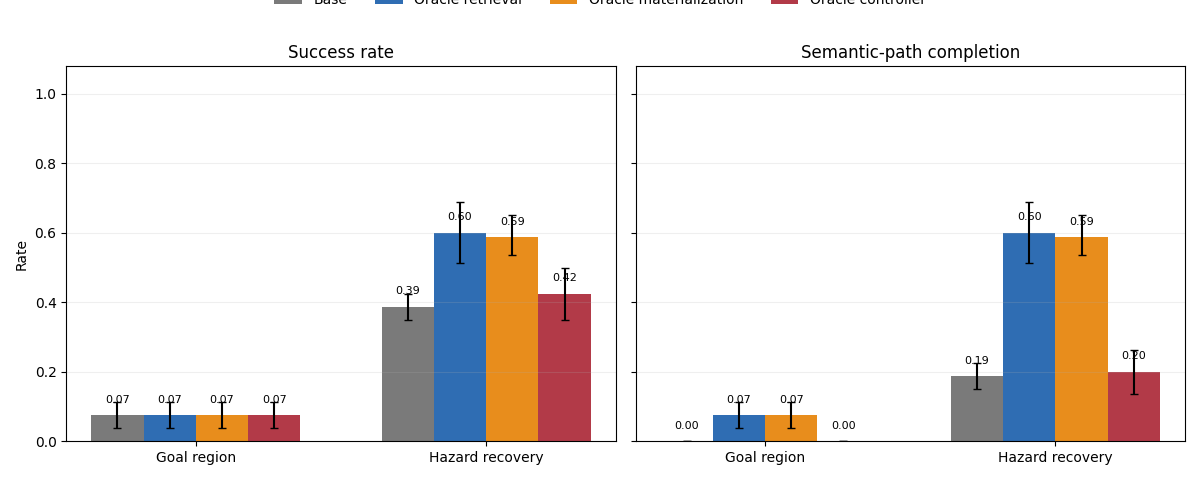
\includegraphics[width=0.84\linewidth]{songlines_symbolic_memory_figures/article_oracle_stage_interventions.png}
  \caption{Oracle-stage interventions on the two hardest task families. Left: end-to-end success. Right: semantic-path completion. Hazard recovery responds strongly to oracle retrieval and oracle materialization, supporting a retrieval/materialization bottleneck. Goal-region remains flat in end-to-end success, but semantic-path completion increases under retrieval/materialization repair, showing that local semantic-path repair is not sufficient to recover full task completion.}
  \label{fig:oracle}
\end{figure*}

\section{Failure analysis}

The framework supports asymmetric failure attribution. Goal-region rejoin is a downstream failure: oracle retrieval and oracle materialization lift semantic-path completion to 0.08 on FourRooms, yet end-to-end success stays flat at 0.08, implying the bottleneck is in handoff/execution after candidate selection. Hazard recovery is the opposite: oracle retrieval/materialization yield +0.20--0.21 success while oracle controller yields only +0.04, locating the bottleneck in semantic selectivity of recovery places, not in last-mile control. Without stage decomposition, both tasks would simply look weak.

\section{Discussion}

The experiments support a qualified yes to the original question: semantic place retrieval can work without coordinate goals, and on harder tasks the framework localizes \emph{where} the pipeline breaks. Water and rest are strong end-to-end cases; goal-region and hazard recovery are not, but they fail for different reasons, and the oracle block confirms those reasons counterfactually. An assist on/off ablation (Appendix~F) further supports the stage-structured reading of Figure~\ref{fig:causal}: assists primarily affect materialization and post-retrieval completion rather than query formation.

The learned behavior-cloned baseline is the cleanest argument for the framework. It reaches 1.00 success on the easiest resource tasks and 0.74 on hazard recovery, but exposes no meaningful intermediate failure states. The Q/R/M/C decomposition is therefore not a competing leaderboard metric; it is the diagnostic layer that becomes essential precisely where success-only evaluation stops being explanatory --- turning semantic-place navigation from an anecdotal systems result into a measurable research problem.

\section{Broader impacts}

The paper is primarily about diagnostic evaluation in simulated navigation environments, so its most immediate positive impact is methodological: it can make memory-based agent failures more measurable and therefore easier to debug, compare, and report honestly. Potential negative impacts are indirect and would arise mainly if similar diagnostic tools were used to improve agents deployed in safety-critical navigation or robotics settings without adequate safeguards. We therefore view the current work as benchmark-level infrastructure rather than as a deployment-ready navigation system.

\section{Limitations and future work}

\textbf{Environment difficulty:} most evidence still comes from MiniGrid; BabyAI appears only as a portability check (Appendix~D). \textbf{Observable-query assumption:} under hidden in-episode query rewrites, the factorization is a projection onto logged traces rather than a full structural claim. \textbf{Oracle-only loop closure:} we close the diagnose$\rightarrow$intervene$\rightarrow$verify loop through oracle interventions, not yet through a retrained v2 retrieval module. \textbf{Baseline scope:} the current baseline set is lightweight; an explicit-memory LLM-agent baseline remains the most important missing comparison.

\begin{ack}
This manuscript is prepared in anonymized form for review. The reported experiments were run from a unified benchmark pipeline that exports task-family summaries, assist on/off comparisons, method diagnostics, and retrieval/control funnels from the same source-of-truth benchmark artifacts.
\end{ack}

{\small
\begin{thebibliography}{9}

\bibitem[Tolman(1948)]{tolman1948cognitive}
E.~C. Tolman.
\newblock Cognitive maps in rats and men.
\newblock \emph{Psychological Review}, 55(4):189--208, 1948.

\bibitem[O'Keefe and Nadel(1978)]{okeefe1978hippocampus}
J.~O'Keefe and L.~Nadel.
\newblock \emph{The Hippocampus as a Cognitive Map}.
\newblock Oxford University Press, 1978.

\bibitem[Kuipers(2000)]{kuipers2000spatial}
B.~Kuipers.
\newblock The spatial semantic hierarchy.
\newblock \emph{Artificial Intelligence}, 119(1--2):191--233, 2000.

\bibitem[Gupta et~al.(2017)]{gupta2017cognitive}
S.~Gupta, J.~Davidson, S.~Levine, R.~Sukthankar, and J.~Malik.
\newblock Cognitive mapping and planning for visual navigation.
\newblock In \emph{Proceedings of the IEEE Conference on Computer Vision and Pattern Recognition}, 2017.

\bibitem[Dayan(1993)]{dayan1993improving}
P.~Dayan.
\newblock Improving generalization for temporal difference learning: The successor representation.
\newblock \emph{Neural Computation}, 5(4):613--624, 1993.

\bibitem[Andrychowicz et~al.(2017)]{andrychowicz2017hindsight}
M.~Andrychowicz, F.~Wolski, A.~Ray, J.~Schneider, R.~Fong, P.~Welinder, B.~McGrew, J.~Tobin, P.~Abbeel, and W.~Zaremba.
\newblock Hindsight experience replay.
\newblock In \emph{Advances in Neural Information Processing Systems}, 2017.

\bibitem[Savinov et~al.(2018)]{savinov2018semi}
N.~Savinov, A.~Dosovitskiy, and V.~Koltun.
\newblock Semi-parametric topological memory for navigation.
\newblock In \emph{International Conference on Learning Representations}, 2018.

\bibitem[Stachenfeld et~al.(2017)]{stachenfeld2017hippocampus}
K.~L. Stachenfeld, M.~M. Botvinick, and S.~J. Gershman.
\newblock The hippocampus as a predictive map.
\newblock \emph{Nature Neuroscience}, 20(11):1643--1653, 2017.

\bibitem[Momennejad et~al.(2017)]{momennejad2017successor}
I.~Momennejad, E.~M. Russek, J.~H. Cheong, M.~M. Botvinick, N.~Daw, and S.~J. Gershman.
\newblock The successor representation in human reinforcement learning.
\newblock \emph{Nature Human Behaviour}, 1:680--692, 2017.

\bibitem[Ghosh et~al.(2021)]{ghosh2021learning}
D.~Ghosh, A.~Gupta, A.~Reddy, J.~Fu, S.~Levine, and C.~Finn.
\newblock Learning to reach goals via iterated supervised learning.
\newblock In \emph{International Conference on Learning Representations}, 2021.

\bibitem[Kolve et~al.(2017)]{kolve2017ai2thor}
E.~Kolve, R.~Mottaghi, D.~Gordon, Y.~Zhu, A.~Gupta, A.~Farhadi, and D.~Fox.
\newblock AI2-THOR: An interactive 3D environment for visual AI.
\newblock \emph{arXiv preprint arXiv:1712.05474}, 2017.

\bibitem[Savva et~al.(2019)]{savva2019habitat}
M.~Savva, A.~Kadian, O.~Maksymets, Y.~Zhao, E.~Wijmans, B.~Jain, J.~Straub, J.~Liu, V.~Koltun, J.~Malik, et al.
\newblock Habitat: A platform for embodied AI research.
\newblock In \emph{Proceedings of the IEEE/CVF International Conference on Computer Vision}, 2019.

\bibitem[Deitke et~al.(2022)]{deitke2022procthor}
M.~Deitke, E.~V. Wijmans, D.~Schwenk, O.~Salvador, K.~M. Ehsani, W.~Han, E.~Vandenschrick, A.~Herrasti, X.~Puig, A.~Farhadi, et al.
\newblock ProcTHOR: Large-scale embodied AI using procedural generation.
\newblock In \emph{Advances in Neural Information Processing Systems Datasets and Benchmarks Track}, 2022.

\bibitem[Wang et~al.(2023)]{wang2023voyager}
G.~Wang, Y.~Xie, Z.~Jiang, A.~Mandlekar, C.~Xie, A.~Yu, and P.~Liang.
\newblock Voyager: An open-ended embodied agent with large language models.
\newblock \emph{arXiv preprint arXiv:2305.16291}, 2023.

\bibitem[Shinn et~al.(2023)]{shinn2023reflexion}
N.~Shinn, F.~Cassano, A.~Berman, and A.~G. Labash.
\newblock Reflexion: Language agents with verbal reinforcement learning.
\newblock In \emph{Advances in Neural Information Processing Systems}, 2023.

\bibitem[Packer et~al.(2023)]{packer2023memgpt}
C.~Packer, V.~Fang, S.~Patil, K.~Lin, S.~Wooders, and J.~Gonzalez.
\newblock MemGPT: Towards LLMs as operating systems.
\newblock \emph{arXiv preprint arXiv:2310.08560}, 2023.

\bibitem[Chevalier-Boisvert et~al.(2018)]{chevalier2018babyai}
M.~Chevalier-Boisvert, D.~Bhoopchand, H.~Abdolmaleki, and A.~Mordatch.
\newblock BabyAI: A platform to study the sample efficiency of grounded language learning.
\newblock In \emph{International Conference on Learning Representations}, 2019.

\bibitem[Chevalier-Boisvert et~al.(2023)]{MinigridMiniworld23}
M.~Chevalier-Boisvert, B.~Lahlou, S.~Willems, and P.~S. Castro.
\newblock MiniGrid and MiniWorld: Modular \& customizable reinforcement learning environments for goal-oriented tasks.
\newblock \emph{arXiv preprint arXiv:2306.13831}, 2023.

\end{thebibliography}
}

\appendix

\section{Formal proof of Theorem~1}

We restate the theorem in the notation used by the benchmark. For each episode $i \in \{1,\dots,n\}$, let
\[
Q_i^\star,\quad R_i^\star,\quad M_i^\star,\quad C_i^\star
\]
denote the nested episode-level indicators defined in Appendix~B. By construction these are measurable functions of the runtime trajectory log for episode $i$ and satisfy
\[
C_i^\star \Rightarrow M_i^\star \Rightarrow R_i^\star \Rightarrow Q_i^\star .
\]

Define the empirical estimators
\[
\hat p_Q = \frac{1}{n}\sum_{i=1}^n Q_i^\star,
\qquad
\hat p_{R\mid Q} = \frac{\sum_{i=1}^n R_i^\star}{\sum_{i=1}^n Q_i^\star},
\]
\[
\hat p_{M\mid R} = \frac{\sum_{i=1}^n M_i^\star}{\sum_{i=1}^n R_i^\star},
\qquad
\hat p_{C\mid M} = \frac{\sum_{i=1}^n C_i^\star}{\sum_{i=1}^n M_i^\star},
\]
with positivity guaranteeing non-zero denominators on the support of the benchmark.

\paragraph{Identifiability.}
Under the conditional stage-Markov assumption, the probability of each next-stage success depends only on the current successful stage, the active query, and the current memory state. The four quantities
\[
P(Q^\star=1),\quad
P(R^\star=1 \mid Q^\star=1),\quad
P(M^\star=1 \mid R^\star=1),\quad
P(C^\star=1 \mid M^\star=1)
\]
are therefore ordinary conditional Bernoulli probabilities over measurable events in the trajectory sigma-algebra. Because the benchmark logs expose those events directly, the factors are identifiable from trajectory observations.

\paragraph{Consistency.}
Assume that benchmark episodes are sampled independently under a fixed experimental condition. Then each indicator sequence $\{Q_i^\star\}_{i=1}^n$, $\{R_i^\star\}_{i=1}^n$, $\{M_i^\star\}_{i=1}^n$, and $\{C_i^\star\}_{i=1}^n$ is i.i.d.\ Bernoulli (or conditionally Bernoulli after restriction to the relevant support event). By the strong law of large numbers,
\[
\frac{1}{n}\sum_{i=1}^n Q_i^\star \to P(Q^\star=1)
\quad\text{almost surely,}
\]
and analogously for the joint indicators $\mathbb{1}[R_i^\star \wedge Q_i^\star]$, $\mathbb{1}[M_i^\star \wedge R_i^\star]$, and $\mathbb{1}[C_i^\star \wedge M_i^\star]$. Positivity implies that the denominators converge almost surely to strictly positive limits, so the continuous mapping theorem gives
\[
\hat p_{R\mid Q} \to P(R^\star=1 \mid Q^\star=1),\quad
\hat p_{M\mid R} \to P(M^\star=1 \mid R^\star=1),\quad
\hat p_{C\mid M} \to P(C^\star=1 \mid M^\star=1)
\]
almost surely. Hence all four empirical stage estimators are consistent.

\paragraph{Product estimator.}
Because the events are nested,
\[
P(C^\star=1)
=
P(Q^\star=1)\,
P(R^\star=1 \mid Q^\star=1)\,
P(M^\star=1 \mid R^\star=1)\,
P(C^\star=1 \mid M^\star=1).
\]
Replacing each factor by its consistent empirical estimator yields a consistent estimator for semantic-path completion, which is the quantity audited in Section~7.1.

\section{Operational vs.\ nested stage estimators}
\label{app:estimators}

The paper uses two related measurement layers.

\paragraph{Operational diagnostic rates.}
The main benchmark logs per-query and per-episode diagnostic quantities directly from runtime traces. A \emph{query formed rate} is the fraction of query attempts with a non-empty candidate set. A \emph{retrieval satisfied rate} is the fraction of query attempts whose selected candidate satisfies the active semantic predicate. A \emph{target materialized rate} is the fraction of query attempts that yield an actionable target. Finally, \emph{completion after retrieval} is an episode-level indicator equal to one when the episode succeeds after at least one materialized semantic target. These are the values reported in the broad benchmark tables and figures; they are operational rates, not direct multiplicative factors.

\paragraph{Nested stage estimators for factorization.}
For the factorization in Section~4, we instead use episode-level nested events derived from the first failure stage recorded in the runtime taxonomy. Let $Q^\star$ denote that the semantic-query stage was entered at least once in the episode, $R^\star$ that the episode advanced beyond retrieval failure, $M^\star$ that at least one semantic target was materialized after retrieval succeeded, and $C^\star$ that the episode completed after such materialization. These events are nested by construction:
\[
C^\star \Rightarrow M^\star \Rightarrow R^\star \Rightarrow Q^\star.
\]
The consistency audit in Section~7.1 reports
\[
\hat P(Q^\star),\quad
\hat P(R^\star \mid Q^\star),\quad
\hat P(M^\star \mid R^\star),\quad
\hat P(C^\star \mid M^\star),
\]
their product, and its gap to semantic-path completion.

\section{Memory and task schema}
\label{app:schemas}

This appendix expands the brief description of the memory stack from Section~5.2 with the per-entity schemas used by the benchmark runner.

\paragraph{Symbolic place records.}
Per-place fields: \texttt{tag\_confidences} (Dirichlet-style posteriors over semantic tags), \texttt{tag\_counts}, \texttt{visit\_count}, \texttt{last\_seen\_step}, \texttt{geometry\_summary}, and an aggregate \texttt{confidence} score. Places are queryable semantic hypotheses, not just trajectory fragments.

\paragraph{Transition records.}
Directed edges $(p_i \to p_j)$ store \texttt{success\_rate}, \texttt{risk\_estimate}, \texttt{cost\_fast}, \texttt{cost\_slow}, and \texttt{freshness}. The fast/slow split lets the planner reason about both reactive and consolidated routing.

\paragraph{Episode records.}
Compact traces with \texttt{intent}, \texttt{state\_summary}, and \texttt{outcome} attached to each visited place; this is what makes retrieval state-aware rather than purely descriptive.

\paragraph{Concept and relation records.}
Cluster identifiers and relation tags linking place records to higher-level categories (for example, \texttt{water-like}, \texttt{post-hazard-rejoin}, \texttt{narrow-corridor}). These are what the planner queries rather than raw places when asked for an intent like \texttt{find\_safe\_rest\_zone}.

The benchmark runner exports task-family summaries with best method and weakest stage, method diagnostics with best task and weakest stage, assist on/off comparisons, and task-wise stage profiles for query, retrieval, materialization, and control. Table~\ref{tab:tasks} below lists the four task families that the main benchmark uses.

\begin{table*}[t]
  \caption{Task families used in the benchmark. All tasks are defined by semantic place patterns rather than explicit coordinate goals.}
  \label{tab:tasks}
  \centering
  \scriptsize
  \setlength{\tabcolsep}{4pt}
  \begin{tabular}{p{1.55cm}p{2.35cm}p{2.1cm}p{5.2cm}}
    \toprule
    Task family & Intent type & Environment(s) & Semantic target description \\
    \midrule
    Water & \texttt{find\_water\_source} & \texttt{Empty-6x6} & Water-associated resource places with accessibility constraints. \\
    Rest & \texttt{find\_safe\_rest\_zone} & \texttt{Empty-6x6} & Low-risk rest places used when agent energy is low. \\
    Goal region & \texttt{find\_goal\_region} & \texttt{Empty-6x6}, \texttt{FourRooms} & Places associated with goal-region evidence rather than a fixed coordinate. \\
    Hazard recovery & \texttt{hazard\_recovery\_exit} & \texttt{LavaGapS7} & Exit-like recovery places that help the agent leave hazard and rejoin navigation. \\
    \bottomrule
  \end{tabular}
\end{table*}

\section{BabyAI portability transfer}
\label{app:babyai}

To probe portability beyond the original MiniGrid task suite, we run a small BabyAI transfer block on \texttt{BabyAI-GoToObjMaze-v0}. This block uses 5 seeds, 8 episodes per seed, and compares \texttt{random}, \texttt{greedy}, \texttt{babyai\_semantic\_node\_v1}, and \texttt{babyai\_semantic\_plan\_v1}. A lightweight wrapper converts BabyAI missions into semantic intents by mapping object types to the existing retrieval tasks, so the same symbolic memory, query logger, and Q/R/M/C bookkeeping can be reused without changing the core stack.

\begin{table*}[t]
  \caption{Preliminary BabyAI \texttt{GoToObjMaze} transfer on 5 seeds. Success remains low for all methods. The greedy baseline reaches 0.175 by exploiting local partial observability without any memory; the semantic variants match this success rate but are the \emph{only} methods that expose non-zero Q/R/M/C traces and build explicit graph memories (83 nodes on average), confirming that this block tests diagnostic portability rather than navigation competitiveness.}
  \label{tab:babyai}
  \centering
  \small
  \setlength{\tabcolsep}{8pt}
  \begin{tabular*}{\textwidth}{@{\extracolsep{\fill}}l c c c c c}
    \toprule
    Method & Success & Query & Retrieval & Materialized & Post \\
    \midrule
    \method{random} & 0.125 & 0.00 & 0.00 & 0.00 & 0.00 \\
    \method{greedy} & 0.175 & 0.00 & 0.00 & 0.00 & 0.00 \\
    \method{babyai-node} & 0.175 & 0.025 & 0.025 & 0.025 & 0.05 \\
    \method{babyai-plan} & 0.175 & 0.025 & 0.025 & 0.025 & 0.05 \\
    \bottomrule
  \end{tabular*}
\end{table*}
\noindent\emph{BabyAI abbreviations:} \method{babyai-node} = \method{babyai\_semantic\_node\_v1}, \method{babyai-plan} = \method{babyai\_semantic\_plan\_v1}.

\begin{figure*}[t]
  \centering
  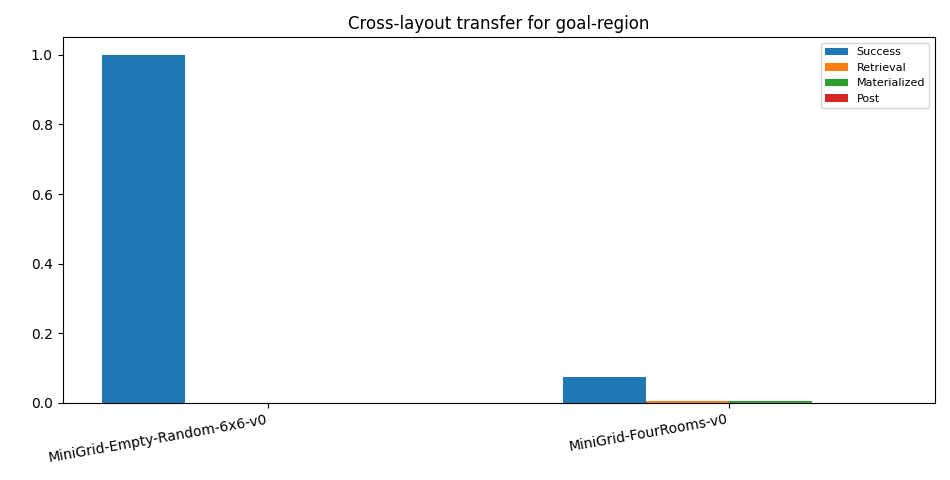
\includegraphics[width=0.82\linewidth]{songlines_symbolic_memory_figures/article_cross_layout.png}
  \caption{Cross-layout transfer for goal-region. Semantic success is near-perfect on Empty-6x6 but collapses on FourRooms, while the bottleneck remains downstream of candidate selection rather than at query formation.}
  \label{fig:cross-layout-appendix}
\end{figure*}

\begin{figure*}[t]
  \centering
  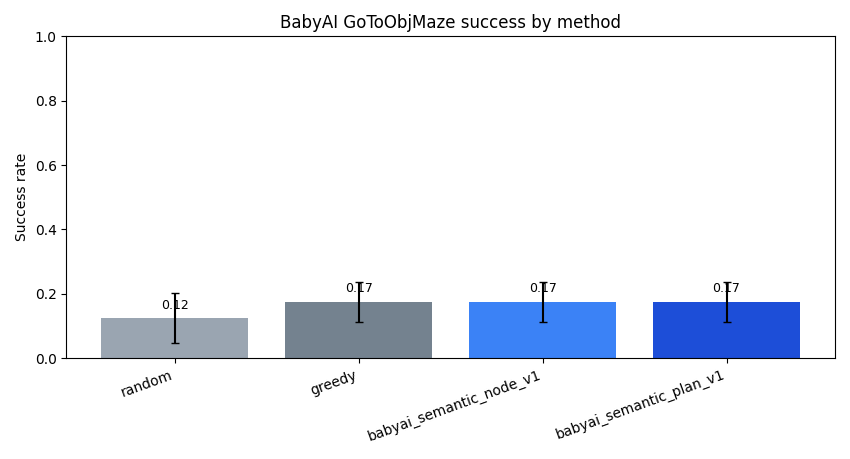
\includegraphics[width=0.72\linewidth]{songlines_symbolic_memory_figures/article_babyai_gotoobjmaze_success.png}
  \caption{Preliminary BabyAI transfer on \texttt{BabyAI-GoToObjMaze-v0}. Random success drops to 0.125, while greedy and both semantic variants reach 0.175. The semantic methods are not stronger in top-line success here, but they remain the only methods that expose non-zero Q/R/M/C traces and build explicit graph memories.}
  \label{fig:babyai-appendix}
\end{figure*}

\section{Extended diagnostics}
\label{app:diagnostics}

\begin{figure*}[t]
  \centering
  \begin{minipage}[t]{0.48\linewidth}
    \centering
    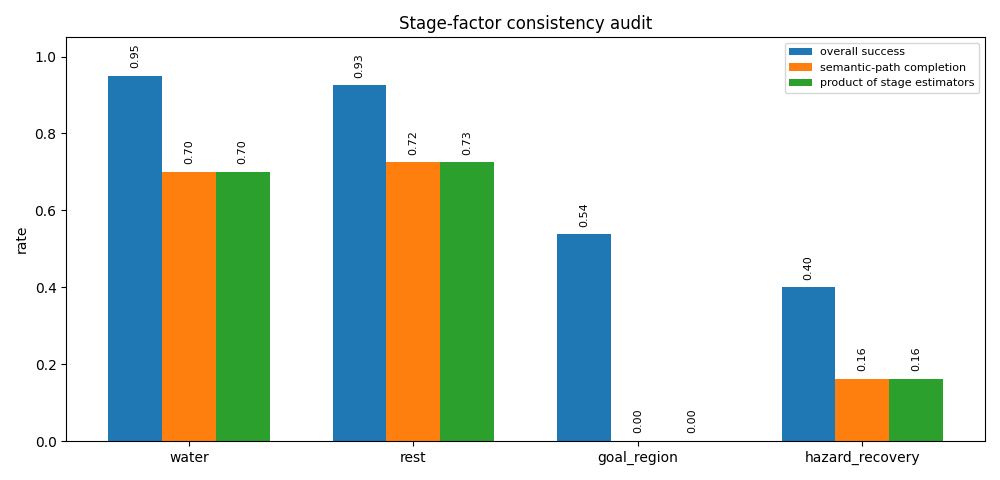
\includegraphics[width=\linewidth]{songlines_symbolic_memory_figures/article_stage_consistency.png}
  \end{minipage}\hfill
  \begin{minipage}[t]{0.48\linewidth}
    \centering
    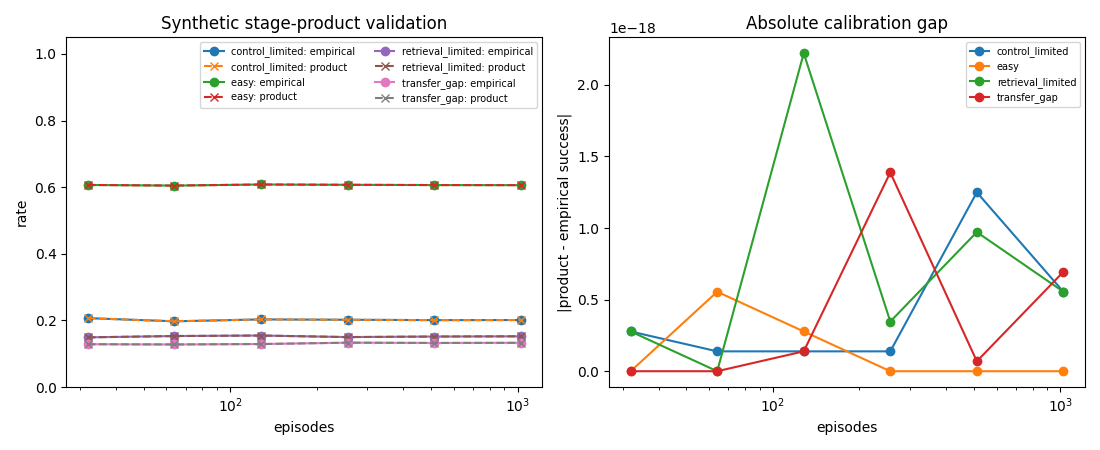
\includegraphics[width=\linewidth]{songlines_symbolic_memory_figures/synthetic_stage_validation.png}
  \end{minipage}
  \caption{Validation of the stage-estimation layer. Left: on real benchmark runs, the product of nested stage estimators matches semantic-path completion rather than overall success. Right: in a synthetic four-stage process with known probabilities, the same estimator product tracks empirical semantic-path completion across sample sizes.}
  \label{fig:stage-validation}
\end{figure*}

\begin{table*}[t]
  \caption{Causal-attribution efficiency from oracle interventions. Efficiency is defined as $\Delta$success divided by oracle activation rate for the corresponding task and regime. For hazard recovery, retrieval/materialization repair is substantially more effective per activation opportunity than controller repair; for goal-region, none of the isolated interventions improves end-to-end success despite high activation of retrieval/materialization repair.}
  \label{tab:attribution}
  \centering
  \small
  \begin{tabular}{p{2.0cm}p{2.2cm}c c c}
    \toprule
    Task & Mode & Activation rate & $\Delta$success & Efficiency \\
    \midrule
    Goal region & Oracle retrieval & 1.00 & +0.00 & 0.00 \\
    Goal region & Oracle materialization & 1.00 & +0.00 & 0.00 \\
    Goal region & Oracle controller & 0.04 & +0.00 & 0.00 \\
    Hazard recovery & Oracle retrieval & 1.00 & +0.21 & 0.21 \\
    Hazard recovery & Oracle materialization & 0.95 & +0.20 & 0.21 \\
    Hazard recovery & Oracle controller & 0.33 & +0.04 & 0.12 \\
    \bottomrule
  \end{tabular}
\end{table*}

\paragraph{Oracle activation and stage deltas.}
Table~\ref{tab:oracle-appendix} makes the oracle block more explicit by reporting how often each oracle actually activated together with the induced changes in semantic-path completion and end-to-end success. The key ambiguity from the main text is now resolved cleanly for goal-region: the retrieval and materialization oracles activate at essentially full rate, yet end-to-end success remains unchanged. Hazard recovery shows the opposite pattern, with large positive deltas once retrieval or materialization is replaced.

\begin{table*}[t]
  \caption{Oracle activation and stage deltas. Activation is the fraction of episodes in which the oracle mechanism was actually used. $\Delta$ values are measured relative to the corresponding base regime for the same task family.}
  \label{tab:oracle-appendix}
  \centering
  \small
  \begin{tabular}{p{1.9cm}p{2.1cm}c c c c c c}
    \toprule
    Task & Mode & Activation & Retrieval (op.) & Materialized (op.) & Semantic-path & $\Delta$ semantic-path & $\Delta$ success \\
    \midrule
    Goal region & Base & --- & 0.02 & 0.02 & 0.00 & 0.00 & 0.00 \\
    Goal region & Oracle retrieval & 1.00 & 0.00 & 1.00 & 0.08 & +0.08 & 0.00 \\
    Goal region & Oracle materialization & 1.00 & 0.02 & 1.00 & 0.08 & +0.08 & 0.00 \\
    Goal region & Oracle controller & 0.04 & 0.01 & 0.01 & 0.00 & 0.00 & 0.00 \\
    Hazard recovery & Base & --- & 0.10 & 0.11 & 0.19 & 0.00 & 0.00 \\
    Hazard recovery & Oracle retrieval & 1.00 & 0.00 & 0.99 & 0.60 & +0.41 & +0.21 \\
    Hazard recovery & Oracle materialization & 0.95 & 0.08 & 0.99 & 0.59 & +0.40 & +0.20 \\
    Hazard recovery & Oracle controller & 0.33 & 0.06 & 0.06 & 0.20 & +0.01 & +0.04 \\
    \bottomrule
  \end{tabular}
\end{table*}

\paragraph{Oracle case studies.}
Figure~\ref{fig:oracle-cases} gives four compact episode-level case studies drawn from the oracle benchmark: a base goal-region failure, a goal-region failure that remains unresolved even after oracle materialization, a base hazard-recovery failure, and a hazard-recovery success rescued by oracle retrieval. These examples make the stage-level diagnosis concrete.

\begin{figure*}[t]
  \centering
  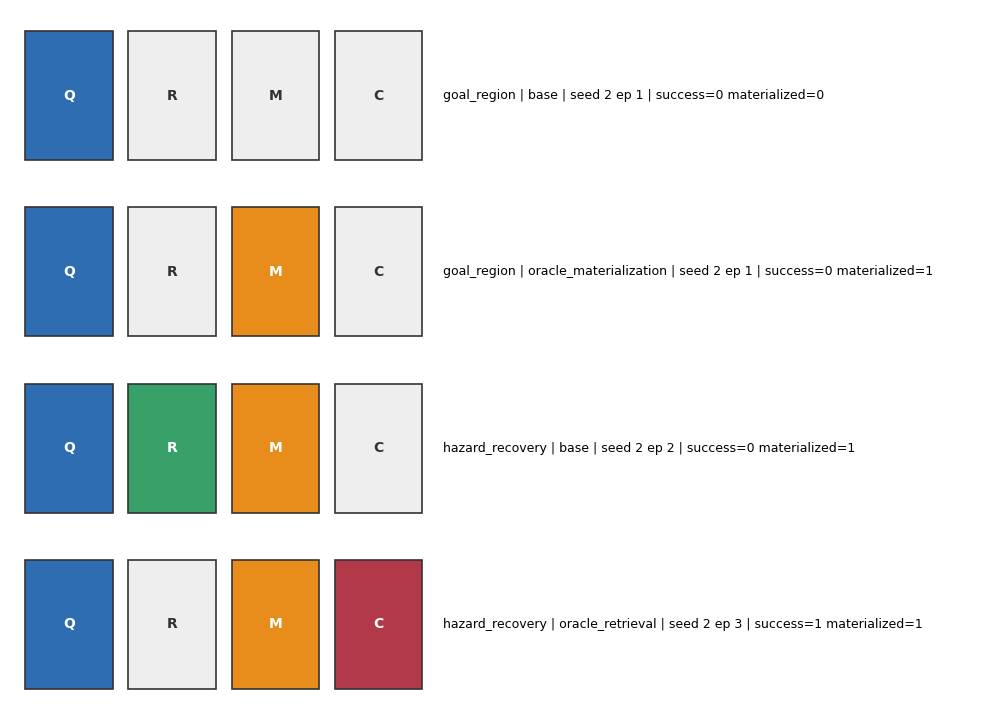
\includegraphics[width=0.84\linewidth]{songlines_symbolic_memory_figures/article_oracle_case_studies.png}
  \caption{Qualitative oracle case studies from the two hardest task families. The panel contrasts cases where local semantic-path repair is sufficient (hazard recovery under oracle retrieval) with cases where it is not (goal-region under oracle materialization).}
  \label{fig:oracle-cases}
\end{figure*}

\begin{figure}[t]
  \centering
  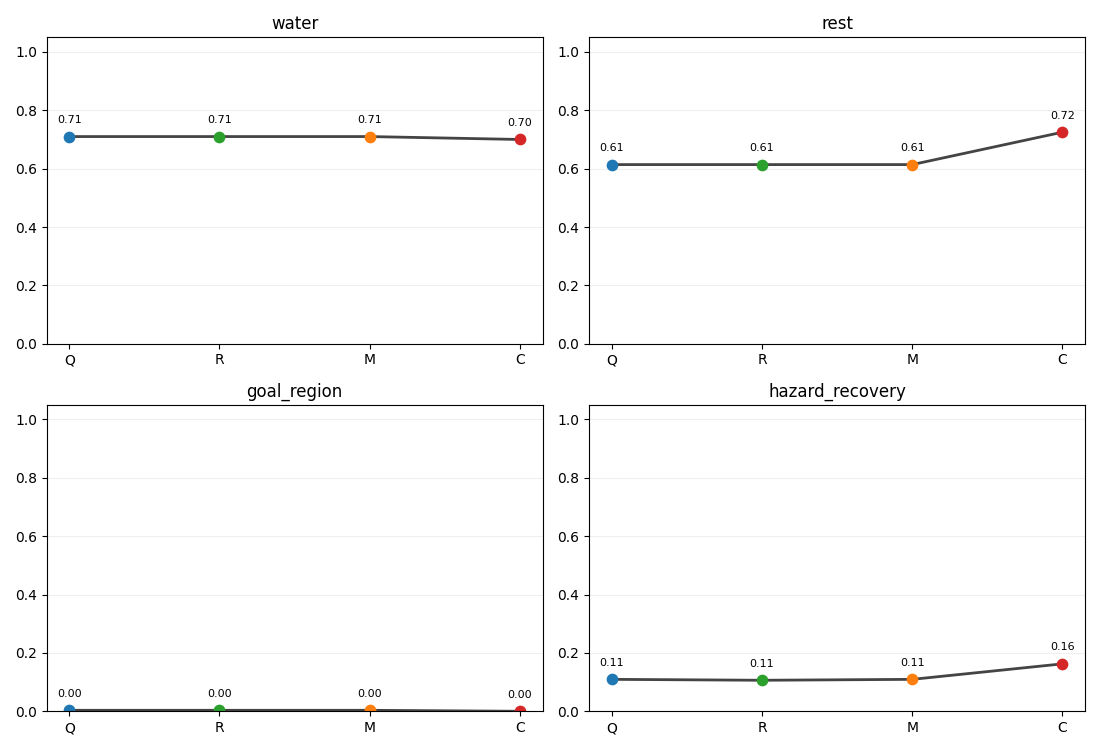
\includegraphics[width=0.88\linewidth]{songlines_symbolic_memory_figures/article_funnel_panel.png}
  \caption{Task-family stage-profile panel moved from the main text. Because these are operational diagnostic rates rather than nested stage estimators, the figure should be read as a profile over stages rather than as a literal monotone funnel.}
  \label{fig:funnels}
\end{figure}

\paragraph{Memory-growth scaling.}
Figure~\ref{fig:scaling-appendix} reports the online memory-growth diagnostic that was removed from the main paper in favor of the stronger oracle-intervention block.

\begin{figure*}[t]
  \centering
  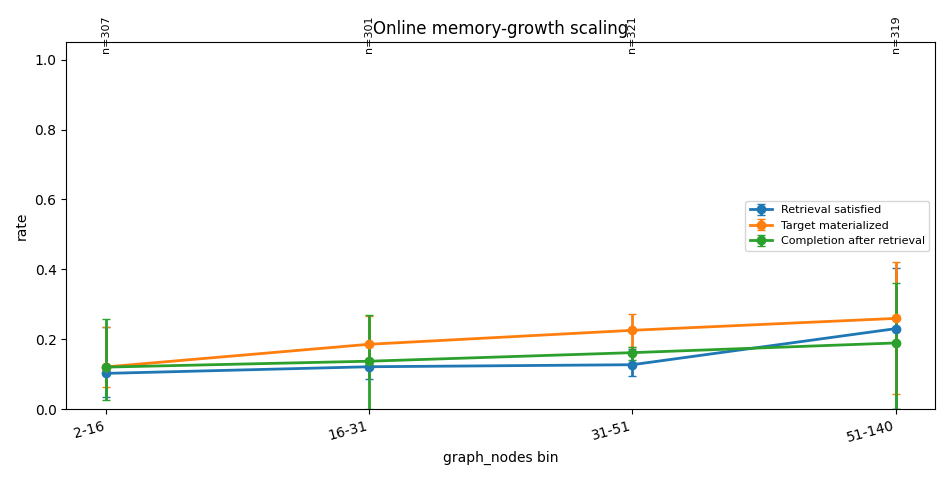
\includegraphics[width=0.82\linewidth]{songlines_symbolic_memory_figures/article_memory_scaling.png}
  \caption{Online memory-growth scaling, shown in the appendix as a descriptive diagnostic trend. Error bars show seed-level bootstrap confidence intervals, and the per-bin sample counts are printed above the x-axis.}
  \label{fig:scaling-appendix}
\end{figure*}

\paragraph{Observation-noise robustness.}
We also ran a targeted robustness sweep over the best semantic variant for each task family under explicit semantic-observation perturbations: tag dropout and false positives in local semantic evidence.

\begin{figure*}[t]
  \centering
  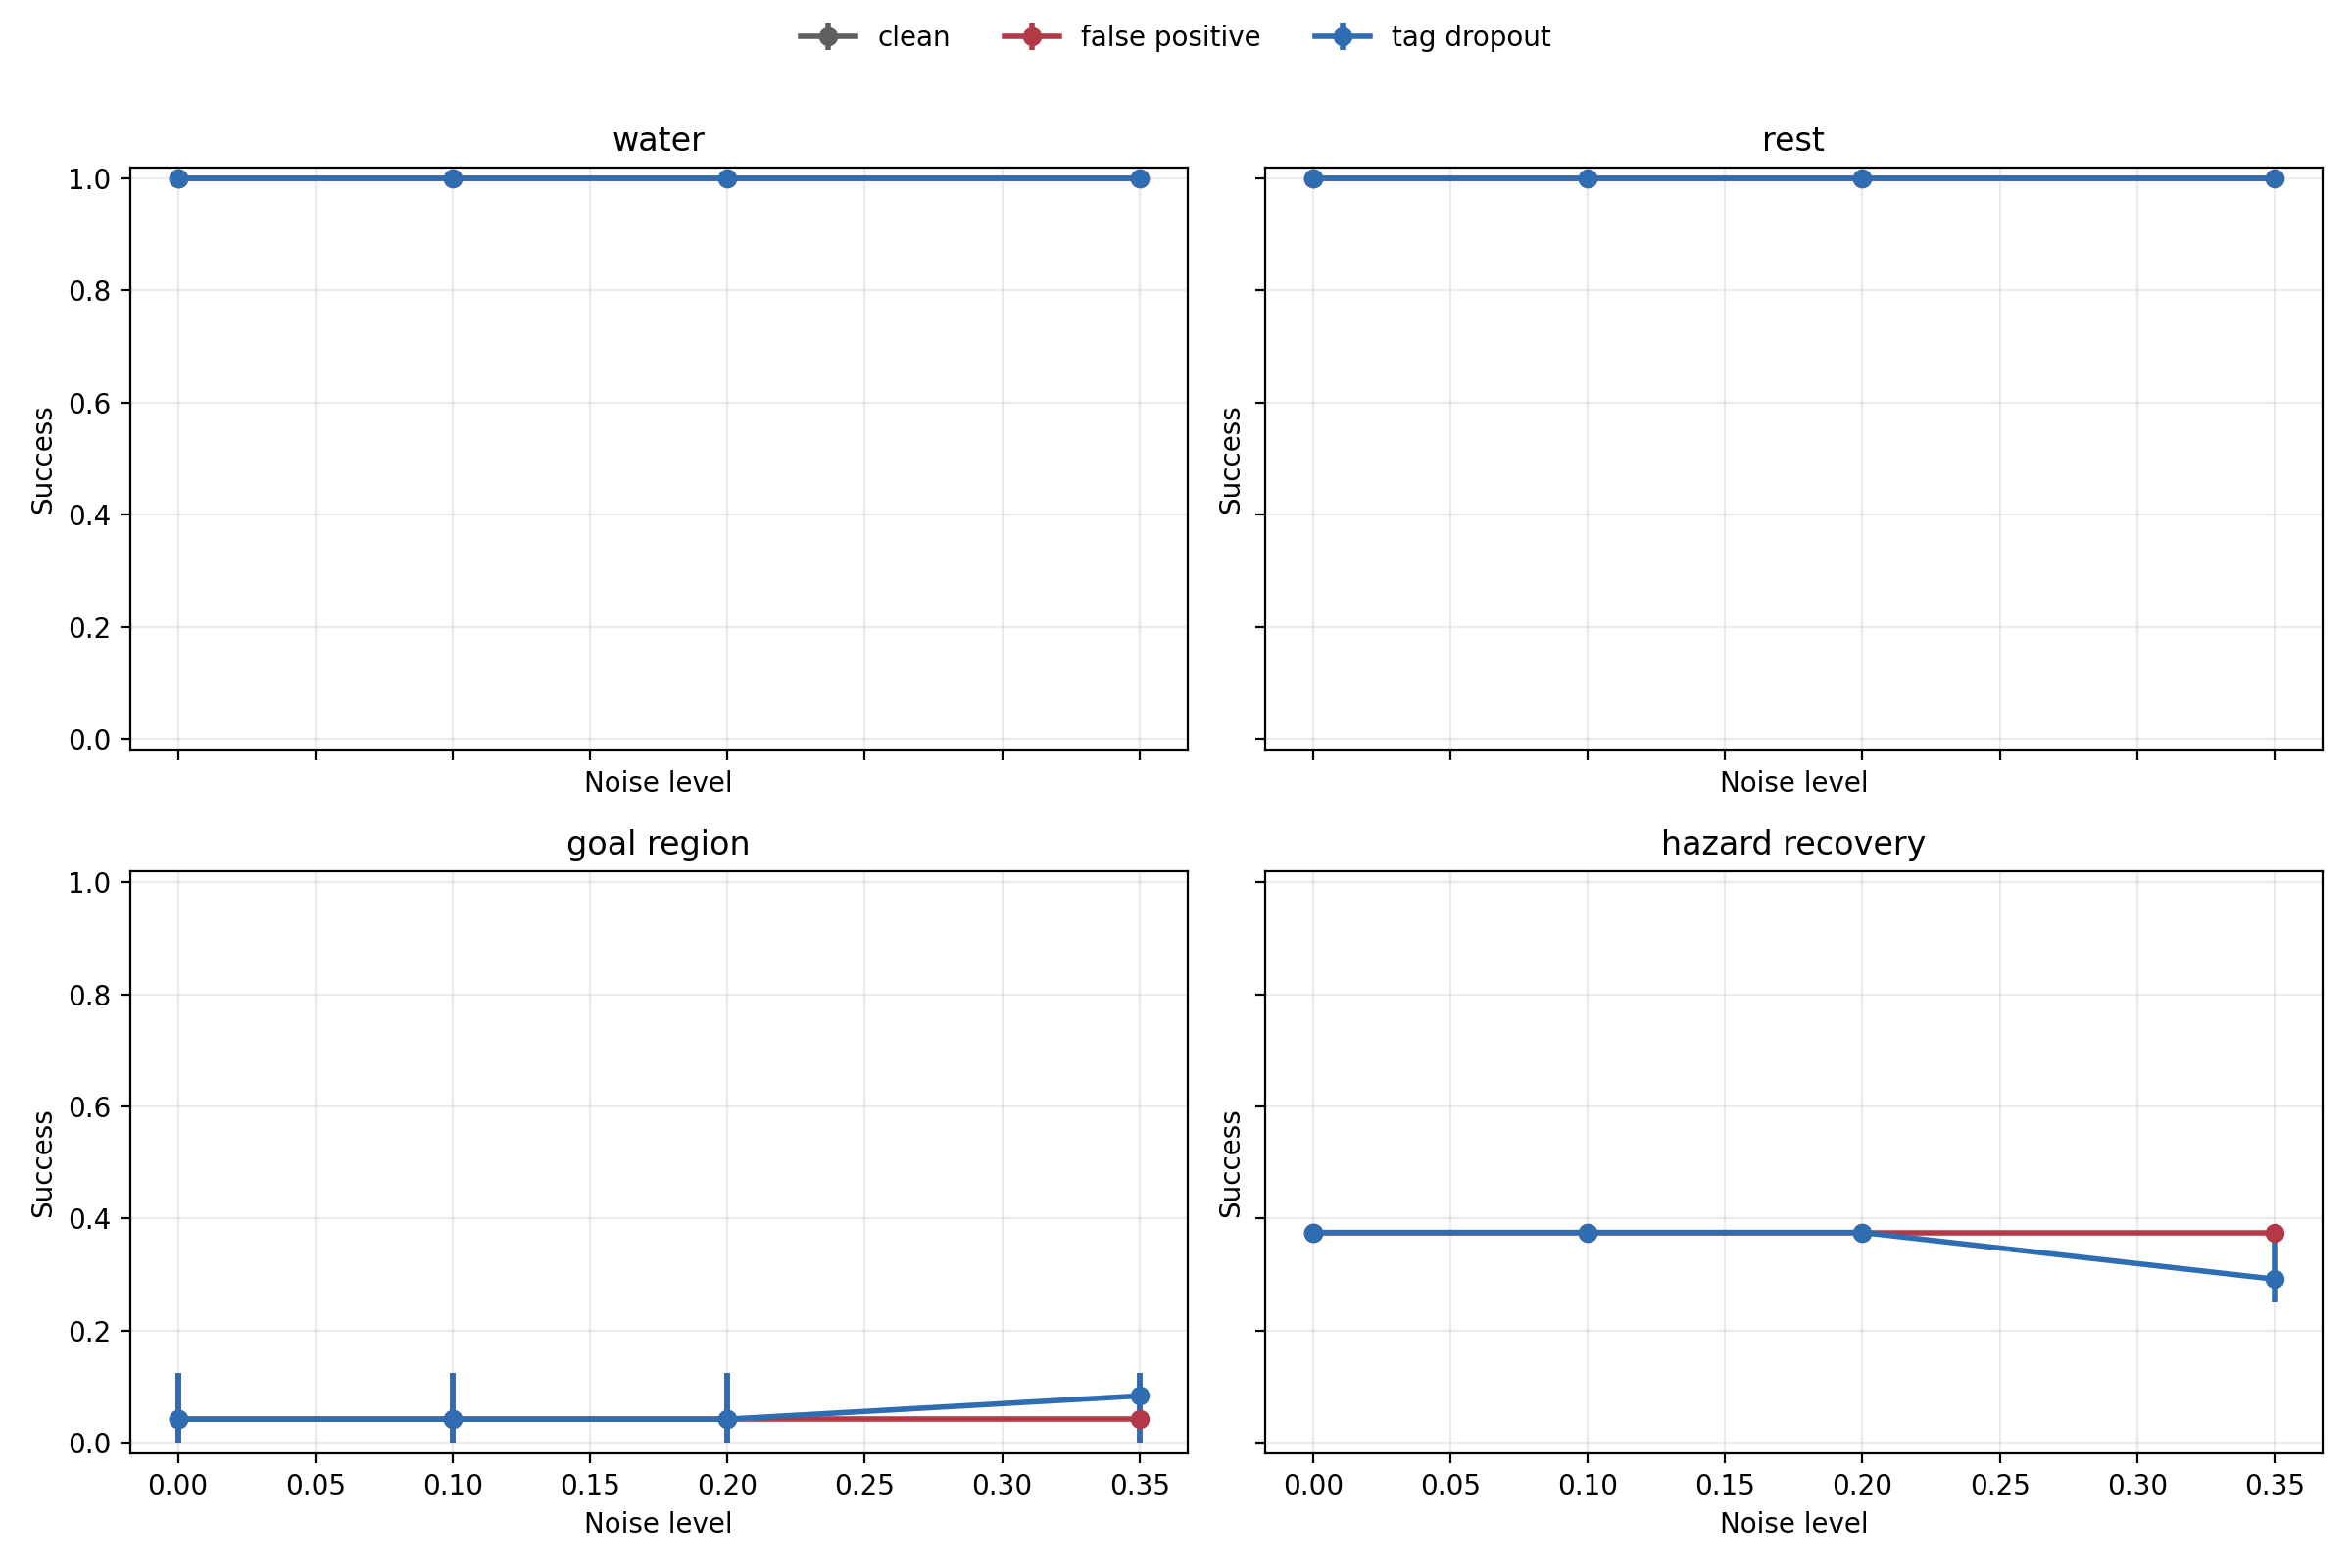
\includegraphics[width=0.84\linewidth]{songlines_symbolic_memory_figures/article_noise_success.png}
  \caption{Success under explicit semantic-observation noise for the best semantic variant in each task family. Water and rest remain stable; hazard recovery is more sensitive, especially under tag dropout; goal-region remains weak but measurable.}
  \label{fig:noise-success}
\end{figure*}

\begin{figure*}[t]
  \centering
  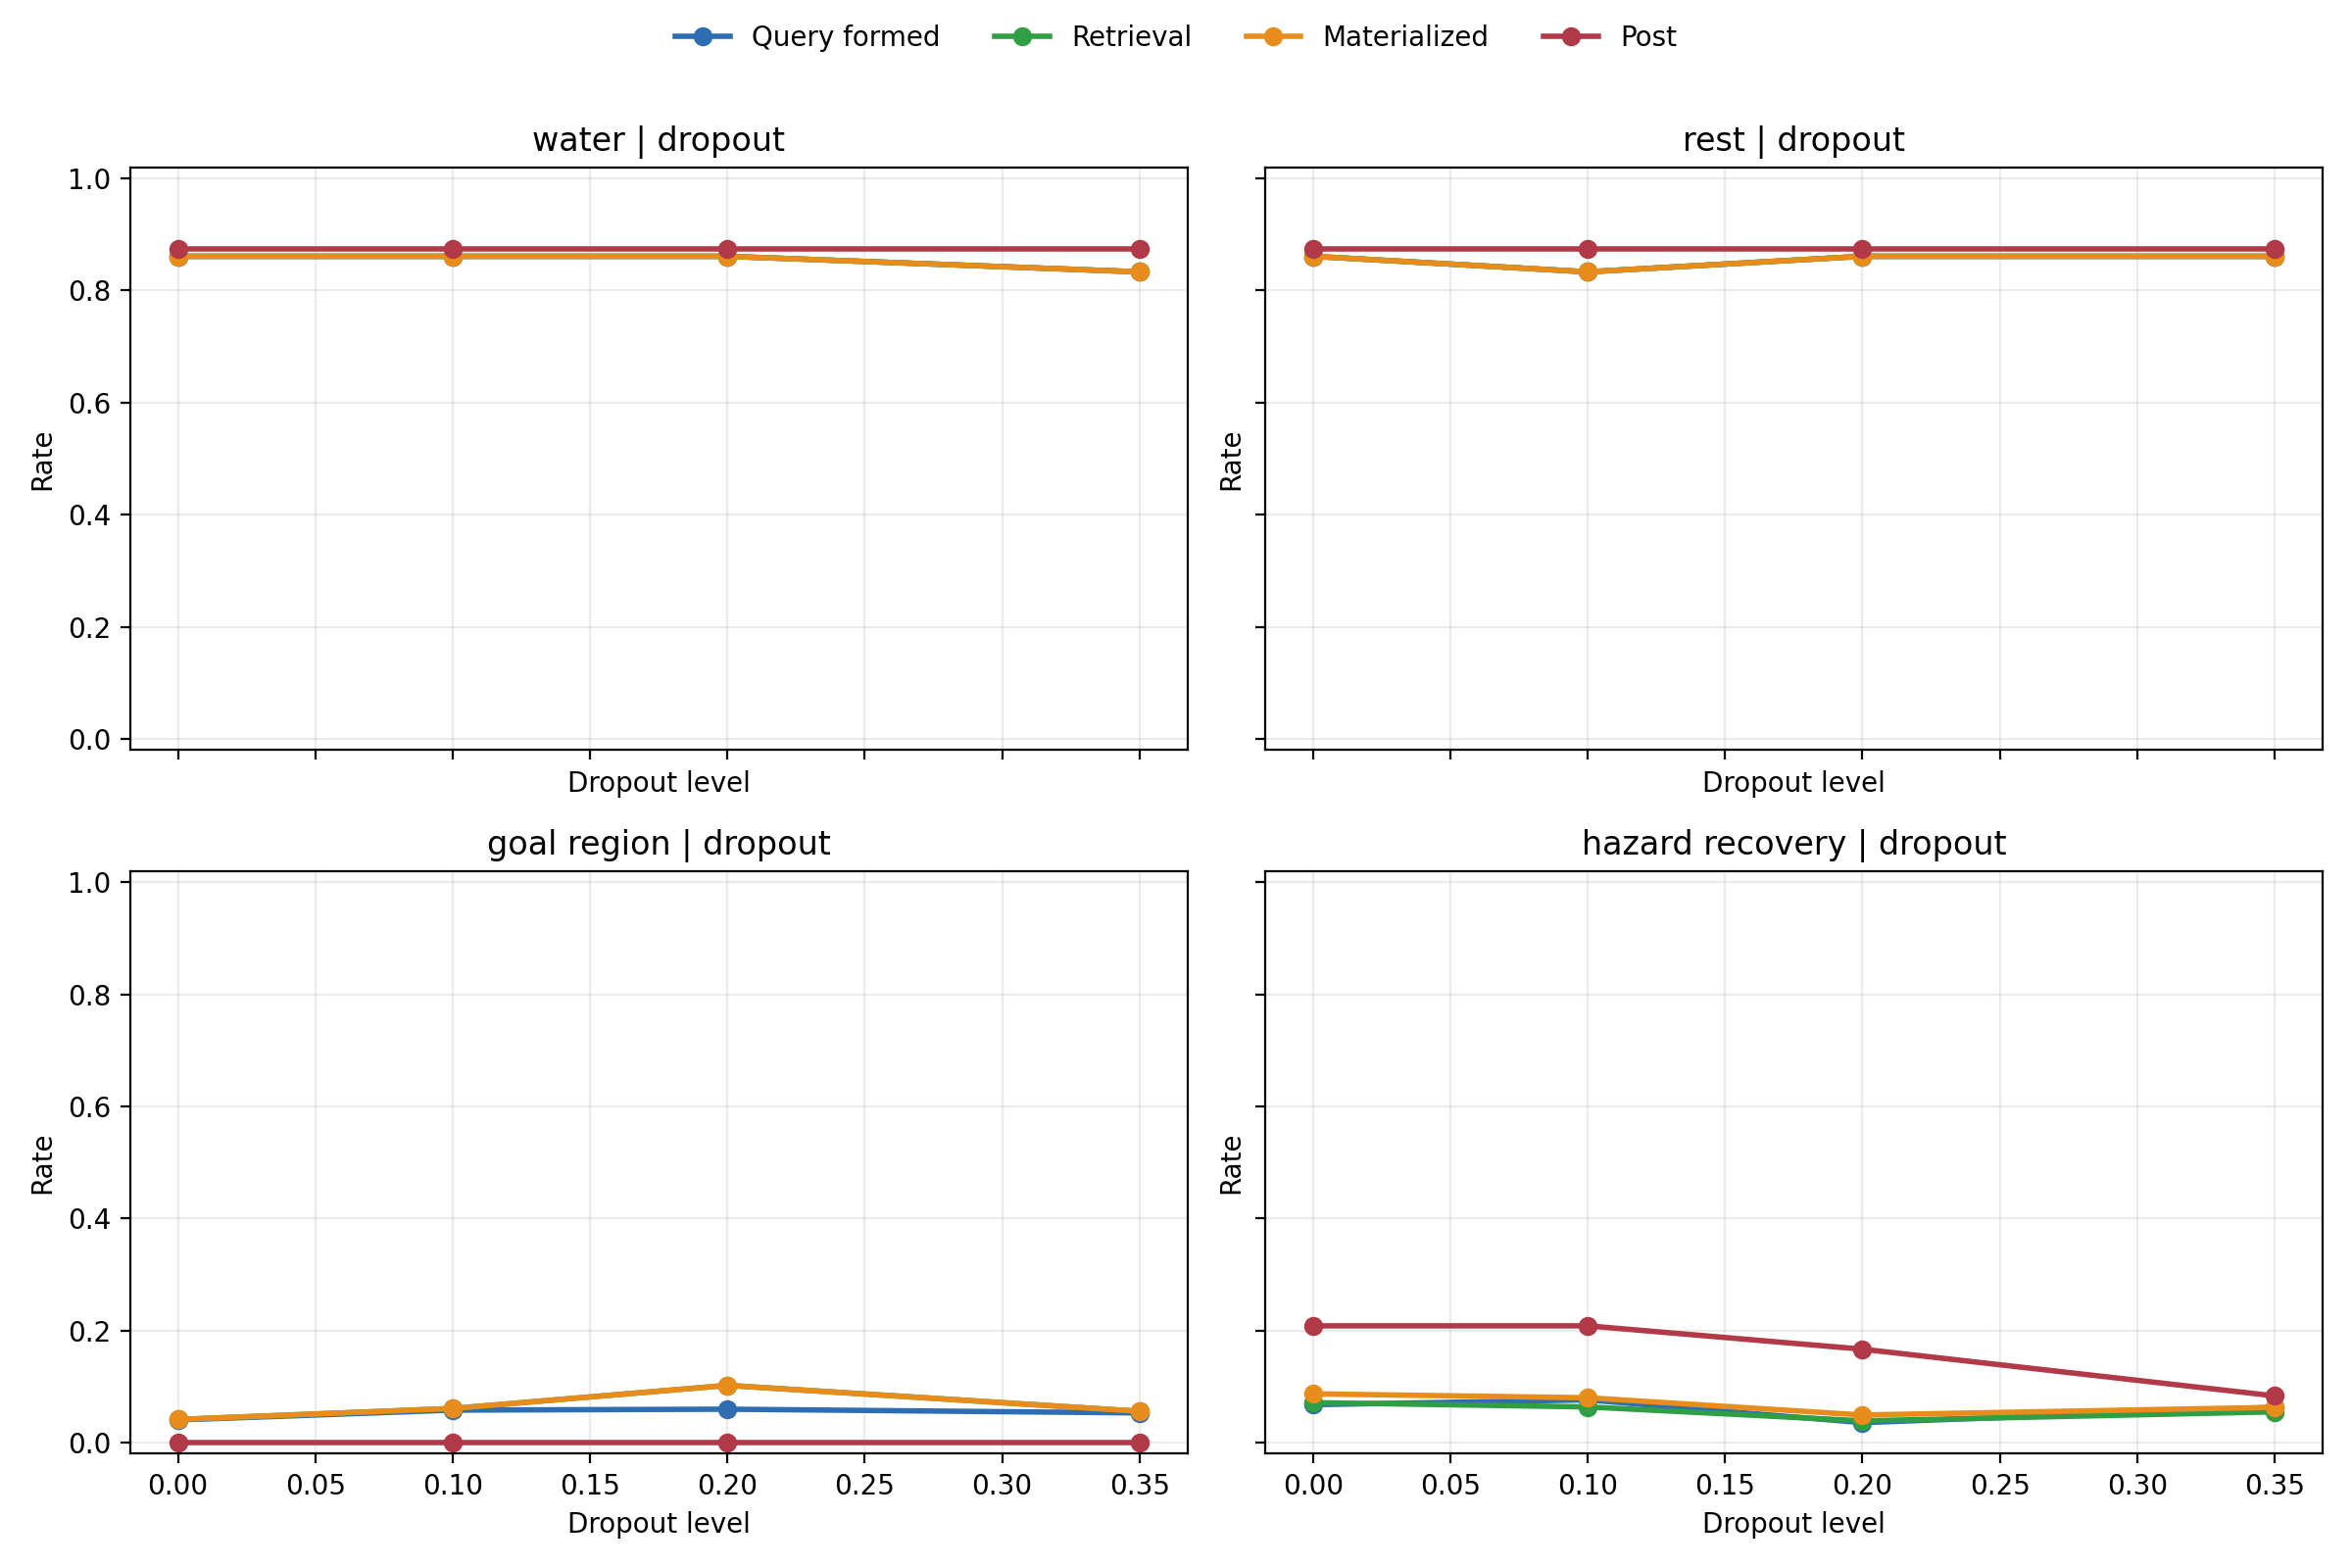
\includegraphics[width=0.84\linewidth]{songlines_symbolic_memory_figures/article_noise_stage_dropout.png}
  \caption{Stage-wise robustness under semantic tag dropout. The curves show how query formation, retrieval, target materialization, and post-retrieval completion change as dropout increases. Hazard recovery degrades early in the pipeline, while the resource tasks remain comparatively flat.}
  \label{fig:noise-stage}
\end{figure*}

\section{Assist on/off analysis}
\label{app:assist}

We include the full assist on/off ablation referenced in Section~9. Across all four task families, top-line success is essentially unchanged ($\Delta \le 0.10$); the only non-trivial effect is on rest, where assists improve post-retrieval completion by~$+0.05$ without changing query/retrieval rates. This supports the stage-structured reading of Figure~\ref{fig:causal}: assists primarily target materialization and post-retrieval execution rather than query formation. Table~\ref{tab:assist} reports the best assist-on versus assist-off result per task family, and Figure~\ref{fig:assist} shows the corresponding paired deltas.

\begin{table*}[t]
  \caption{Best assist-on versus assist-off result per task family. Water is almost unchanged, rest gains top-line success mainly through later completion, goal-region is unchanged, and hazard recovery shifts only slightly between retrieval and post-retrieval completion without changing success.}
  \label{tab:assist}
  \centering
  \scriptsize
  \setlength{\tabcolsep}{3.5pt}
  \begin{tabular}{p{1.6cm}p{1.45cm}p{1.45cm}c c c c p{3.0cm}}
    \toprule
    Task & Best method (on) & Best method (off) & Success on/off & Retrieval on/off & Materialized on/off & Post-retrieval on/off & Main effect \\
    \midrule
    Water & \method{water-cp} & \method{water-cp} & 0.95 / 0.94 & 0.71 / 0.75 & 0.71 / 0.75 & 0.70 / 0.74 & effect is negligible \\
    Rest & \method{rest-s2} & \method{rest-s2} & 0.93 / 0.83 & 0.61 / 0.66 & 0.61 / 0.66 & 0.73 / 0.68 & assists help success mainly downstream \\
    Goal region & \method{goal-n1} & \method{goal-n1} & 0.54 / 0.54 & 0.00 / 0.00 & 0.00 / 0.00 & 0.00 / 0.00 & assists do not change the outcome \\
    Hazard recovery & \method{hazard-s7} & \method{hazard-s7} & 0.40 / 0.40 & 0.11 / 0.11 & 0.11 / 0.11 & 0.16 / 0.15 & only a small stage shift \\
    \bottomrule
  \end{tabular}
\end{table*}

\begin{figure*}[t]
  \centering
  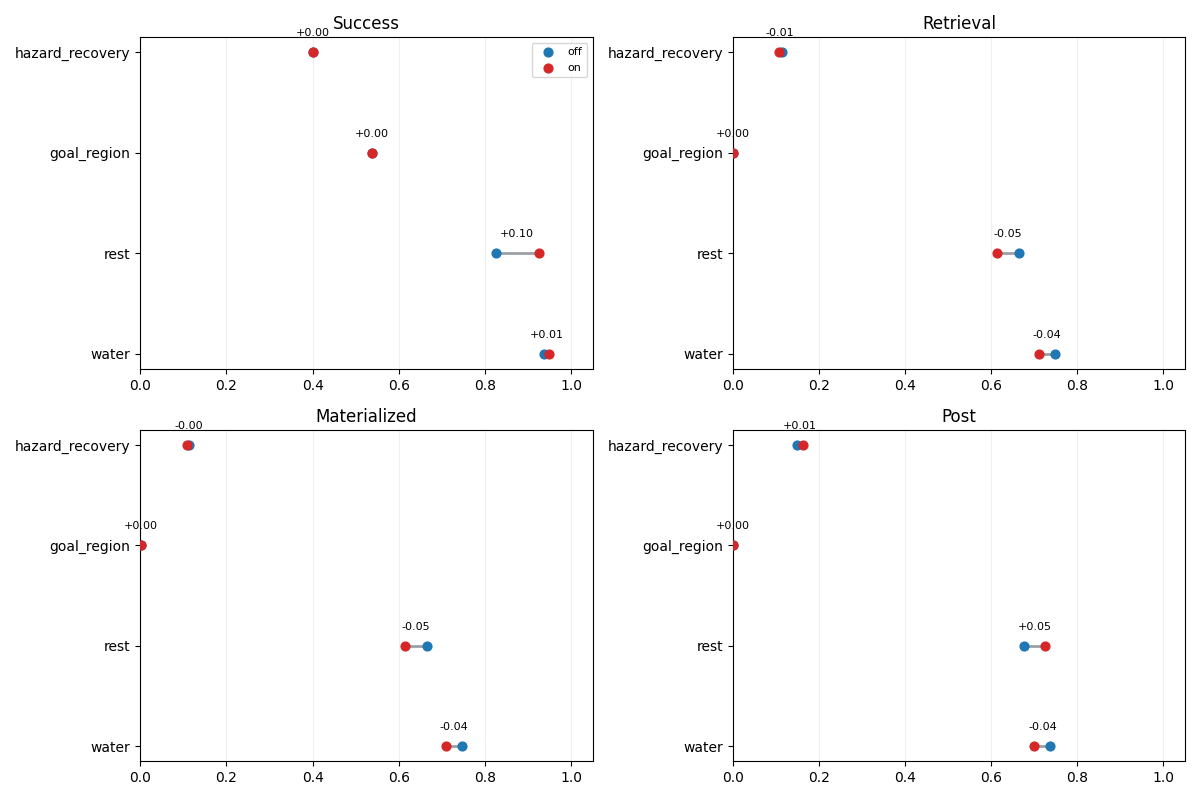
\includegraphics[width=0.88\linewidth]{songlines_symbolic_memory_figures/article_assist_dumbbell.png}
  \caption{Assist on/off comparison shown as paired deltas. Water is essentially unchanged, rest gains most in top-line success, goal-region is unchanged, and hazard recovery shifts failure only slightly later in the pipeline without changing top-line success.}
  \label{fig:assist}
\end{figure*}

\section{Reproducibility commands}
\label{app:repro}

The main paper artifacts were generated from the following benchmark and analysis scripts:
\begin{itemize}[leftmargin=16pt]
\item article benchmark and learned-baseline suite: \path{scripts/benchmark_symbolic_memory_article.py}
\item article analysis and figure generation: \path{scripts/analyze_symbolic_memory_article.py}
\item synthetic factorization sanity check: \path{scripts/validate_qrmc_factorization.py}
\item oracle-stage intervention benchmark: \path{scripts/benchmark_oracle_stage_interventions.py}
\item semantic observation-noise benchmark: \path{scripts/benchmark_semantic_noise_robustness.py}
\item BabyAI transfer benchmark: \path{scripts/compare_songline_babyai.py}
\end{itemize}

\section{Asset and license note}
\label{app:assets}

The experiments use MiniGrid~\citep{MinigridMiniworld23} and BabyAI~\citep{chevalier2018babyai}, both of which are released under the MIT License. The locally implemented baselines and benchmark runner scripts introduced in this paper will be released under the MIT License as part of the camera-ready artifact package. A full version-and-license manifest is being prepared for that release.

\clearpage
\FloatBarrier
\input{checklist.tex}

\end{document}
